\documentclass[../main.tex]{subfiles}

\begin{document}
\chapter{Gewöhnliche Differentialgleichungen}\label{chp:odes}
Bevor wir Differentialgleichungen studieren können,
müssen wir den Raum $\mathbb{R}^n$ besser verstehen.
Wir erinnern uns nun an das Studium von Funktionen
in einer Variable.
Dort machen viele Definitionen
vom Absolutbetrag Gebrauch.

\begin{examples}
  \leavevmode
  \begin{enumerate}[(1)]
    \item Konvergenz einer Folge $a \colon \mathbb{N} \to \mathbb{R}$,
      in Symbolen
      \[
        \lim_{n \to \infty} a(n) = \alpha \in \mathbb{R}
      \]
      heisst folgendes. Für alle $\varepsilon > 0$ existiert
      $N \in \mathbb{N}$ so, dass für alle $n \geq N$ 
      gilt, dass $|a(n) - \alpha| \leq \varepsilon$.
    \item Stetigkeit einer Funktion $f \colon \mathbb{R} \to \mathbb{R}$ 
      im Punkt $p\in \mathbb{R}$ heisst, dass für alle $\varepsilon > 0$ 
      ein $\delta > 0$ existiert, so dass
      für alle $q \in \mathbb{R}$ mit $|q - p| \leq \delta$ gilt,
      dass $|f(q) - f(p)| \leq \varepsilon$.
  \end{enumerate}
\end{examples}

Beide dieser sehr zentralen Konzepte machen kritischen Gebrauch
des Absolutbetrags.
In $\mathbb{R}^n$ gibt es aber keinen kanonischen Ersatz für diesen.
Dies motiviert unseren ersten Abschnitt in diesem Kapitel.

\section{Normen auf reellen Vektorräumen}
Die Normaxiome greifen die wichtigsten Eigenschaften des
Absolutbetrags in $\mathbb{R}$ auf und verallgemeinern
diese, so dass wir in allgemeinen reellen Vektorräumen
Konzepte wie Konvergenz und Stetigkeit formalisieren können.

\begin{definition}
  Sei $V$ ein Vektorraum über $\mathbb{R}$.
  Eine Abbildung $\Vert \cdot \Vert \colon V \to \mathbb{R}$
  heisst \emph{Norm} auf $V$, falls folgende Eigenschaften erfüllt werden.
  \begin{enumerate}[(i)]
    \item (Strikte Positivität)
      Für alle $v \in V$ gilt $\Vert v \Vert \geq 0$ und
      $\Vert v \Vert = 0$ genau dann, wenn $v = 0$.
    \item (Homogenität)
      Für alle $v \in V$ und alle $\lambda \in \mathbb{R}$ gilt
      $\Vert \lambda v \Vert = |\lambda| \cdot \Vert v \Vert$.
    \item (Dreiecksungleichung)
      Für alle $v, w \in V$ gilt $\Vert v + w \Vert \leq \Vert v \Vert
      + \Vert w \Vert$.
  \end{enumerate}
\end{definition}

Eigenschaft (ii) hätten wir auch folgendermassen formulieren können:
Die Norm $\Vert \cdot \Vert$ auf einen eindimensionalen Unterraum
von $V$ verhält sich (bis auf Streckung) genau so wie der Absolutbetrag
auf $\mathbb{R}$.

\begin{definition}
  Sei $\Vert \cdot \Vert$ eine Norm auf einem rellen Vektorraum $V$.
  Die Menge
  \[
    B_1 = \left\{v \in V \mid \Vert v \Vert \leq 1\right\} \subset V
  \]
  heisst \emph{Norm-Einheitsball}.
\end{definition}

\begin{examples}
  Sei $V = \mathbb{R}^n$ mit Standardbasis $e_1, \dots, e_n$.
  Einen Vektor $v \in V$ können wir dann ausdrücken durch
  $v = v_1 e_1 + \cdots + v_n e_n$ mit $v_i \in \mathbb{R}$.
  \begin{enumerate}[(1)]
    \item Die \emph{Summennorm} ist die Norm
      \[
        \Vert v \Vert_1 = |v_1| + \cdots + |v_n|.
      \]
      Wir prüfen nun die Normaxiome.
      \begin{enumerate}[(i)]
        \item Dank den Eigenschaften des
          Absolutsbetrag auf $\mathbb{R}$ haben wir sofort 
          $\Vert v \Vert_1 \geq 0$ 
          und $\Vert v \Vert_1 = 0$ genau dann, wenn alle $v_i$ null sind.
        \item Berechne $\Vert \lambda v \Vert_1
          = |\lambda v_1| + \cdots |\lambda v_n| = |\lambda| \cdot
          \Vert v \Vert_1$.
        \item Berechne
          \begin{align*}
            \Vert v + w \Vert_1
            &= |v_1 + w_1| + \cdots + |v_n + w_n| \\
            & \leq |v_1| + |w_1| + \cdots + |v_n| + |w_n| \\
            &= \Vert v \Vert_1 + \Vert w \Vert_1.
          \end{align*}
      \end{enumerate}
    \item Die \emph{Maximumnorm}
      ist die Norm
      \[
        \Vert v \Vert_{\infty}
        = \max \{ |v_1|, \dots |v_n|\}.
      \]
      Wir prüfen wieder die Normaxiome.
      \begin{enumerate}[(i)]
        \item Wir haben $\Vert v \Vert_{\infty} \geq 0$
          und auch $\Vert v \Vert_{\infty}$ genau dann,
          wenn alle $v_i$ null sind.
        \item Es gilt $\Vert \lambda v \Vert_{\infty}
          = \max \left\{v_1, \dots, v_n\right\} = |\lambda|
          \cdot \Vert v \Vert_\infty$.
        \item Berechne
          \begin{align*}
            \Vert v + w \Vert_\infty
            &= \max \left\{|v_1 + w_1|, \dots |v_n + w_n|\right\} \\
            &\leq \max \left\{|v_{1}|, \dots, |v_{n}|\right\}
            + \max \left\{|w_{1}|, \dots, |w_{n}|\right\} \\
            &= \Vert v \Vert_{\infty} + \Vert w \Vert_{\infty},
          \end{align*}
          da jeweils $|v_i + w_i| \leq |v_i| + |w_i| $ gilt.
      \end{enumerate}
    \item die \emph{euklidische Norm} ist die Norm
      \[
        \Vert v \Vert_2 = \sqrt{v_1^2 + \cdots v_n^2}.
      \]
      Auch für diese Norm prüfen wir die Axiome.
      \begin{enumerate}[(i)]
        \item Es gilt $\Vert v \Vert_2 \geq 0$ und
          $\Vert v \Vert_2 = 0$ genau dann, wenn
          $v_1^2 + \cdots + v_n^2 = 0$ gilt,
          was äquivalent dazu ist, dass alle $v_i$ null sind.
        \item Berechne $\Vert \lambda v \Vert_2 = |\lambda | \cdot
          \Vert v \Vert_2$, da $\sqrt{\lambda^2} = |\lambda|$ gilt.
        \item Hier stossen wir zum ersten mal auf Schwierigkeiten.
          Wir werden das im Lemma unten zeigen.
      \end{enumerate}
    \item 
      Folgendes Beispiel rechtfertigt die Notation
      für obige Normen. Sei $p \geq 1$ für $p \geq 1$.
      Die \emph{$p$-Norm} ist
       \[
         \Vert v \Vert_p = \sqrt[p]{|v_1|^p + \cdots + |v_n|^p}.
      \]
      Die Dreiecksungleichung $\Vert v + w \Vert_p \leq
      \Vert v \Vert_p + \Vert w \Vert_p$ heisst
      \emph{Minkowski-Ungleichung}, die aus der
      Konkavität von $\log$ folgt. Siehe hier Abschnitt
      59.3 in~\cite{heuser}.
      Die Normen $\Vert \cdot \Vert_1$ und $\Vert \cdot \Vert_2$ 
      sind Spezialfälle dieser Familie von Normen.
      Für alle $p \geq 1$ gilt, dass $\Vert v \Vert_{\infty}
      \leq \Vert v \Vert_p \leq \sqrt[p]{n} \Vert v \Vert_{\infty}$.
      Im Grenzwert $p \to \infty$ erhalten wir
      \[
        \lim_{p \to \infty} \Vert v \Vert_p = \Vert v \Vert_{\infty}
      \]
      da $\lim_{p \to \infty} \sqrt[p]{n} = 1$.
  \end{enumerate}
  Die Normbälle der ersten drei Normen im Fall $n = 2$
  sind in Abbildung~\ref{fig:norms}
  zu sehen.
\end{examples}

\begin{figure}[htb] 
  \centering
  \begin{minipage}{0.33\textwidth}
    \centering
    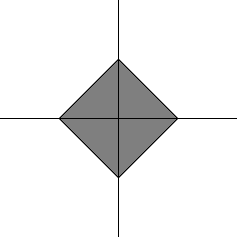
\includegraphics{figures/sumnorm}
  \end{minipage}%
  \begin{minipage}{0.33\textwidth}
    \centering
    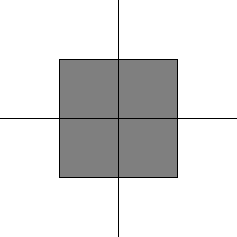
\includegraphics{figures/maxnorm}
  \end{minipage}%
  \begin{minipage}{0.33\textwidth}
    \centering
    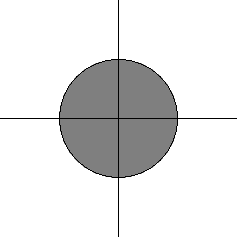
\includegraphics{figures/euclideannorm}
  \end{minipage}%
  \caption{Normbälle der Normen
  $\Vert \cdot \Vert_1,
 \Vert \cdot \Vert_{\infty},
 \Vert \cdot \Vert_2$}%
  \label{fig:norms}
\end{figure}

\subsection*{Normen aus Skalarprodukten}
\begin{definition}
  Ein \emph{Skalarprodukt} auf einem reellen Vektorraum $V$ 
  ist eine strikt positive, symmetrische, bilineare Abbildung
  $\langle \cdot, \cdot \rangle \colon V \times V \to \mathbb{R}$.
  Das heisst,
  \begin{enumerate}[(i)]
    \item für alle $v \in V$ gilt $\langle v, v \geq 0 \rangle$ 
      und $\langle v, v \rangle = 0$ genau dann,
      wenn $v = 0$,
    \item für alle $v, w \in V$ gilt 
      $\langle v, w \rangle = \langle w, v \rangle$,
    \item für alle $u, v, w \in V$ und $t \in \mathbb{R}$ gilt
      $\langle u, v + tw \rangle = \langle u, v \rangle + t
      \langle u, w \rangle$.
  \end{enumerate}
\end{definition}

\begin{lemma*}
  Sei $\langle \cdot, \cdot \rangle$ ein Skalarprodukt auf $V$.
  Dann ist die Abbildung
  \begin{align*}
    \Vert \cdot \Vert \colon V & \to \mathbb{R} \\
    v & \mapsto \sqrt{\langle v, v \rangle}
  \end{align*}
  eine Norm auf $V$.
\end{lemma*}

\begin{proof}
  Wir prüfen die Normaxiome folgendermassen.
  \begin{enumerate}[(i)]
    \item Es gilt $\Vert v \Vert = \sqrt{\langle v, v \rangle} \geq 0$
      und $\Vert v \Vert = 0$ genau dann, wenn
      $\langle v, v \rangle = 0$, das heisst $v = 0$ gilt.
    \item Berechne $\Vert \lambda v \Vert = \sqrt{\langle \lambda v,
      \lambda v\rangle}
      = \sqrt{\lambda^2 \cdot \langle v, v \rangle} = |\lambda| \cdot
      \Vert v \Vert$.
    \item Seien $v, w \in V$. Wir wollen zeigen, dass
      $\sqrt{\langle v + w, v + w \rangle} \leq
      \sqrt{\langle v, v \rangle} + \sqrt{\langle w, w \rangle}$.
      Da Quadrieren auf $\mathbb{R}_{\geq 0}$ monoton ist,
      reicht es zu zeigen, dass
      \[
      \langle v + w, v+ w \rangle\leq \langle v, v \rangle
      + \langle w, w \rangle + 2 \cdot \sqrt{\langle v, v \rangle} \cdot
      \sqrt{\langle w, w \rangle}.
      \]
      Ausmultiplizieren der linken Seite und Subtraktion der Terme,
      die dann auf beiden Seiten erscheinen liefert, dass
      die Dreiecksungleichung für $\Vert \cdot \Vert$ äquivalent
      zur \emph{Cauchy-Schwarz Ungleichung}
      \[
        \langle v, w \rangle \leq \sqrt{\langle v, v \rangle}
        \cdot \sqrt{\langle w, w \rangle}
      \]
      ist.
      Wir beweisen nun diese.
      Betrachte dazu die Funktion $h \colon \mathbb{R} \to \mathbb{R}$,
      die durch
      \[
        h(t) = \langle v + tw, v + tw \rangle \geq 0
      \]
      definiert ist.
      Es gilt also $h(t) = t^2 \langle w, w \rangle + 2t \langle v, w \rangle
      + \langle v, v \rangle$.
      Dies beschreibt eine Parabel mit Diskriminante
      \[
        D = b^2 - 4ac = 4\langle v, w \rangle^2 - 4\langle w, w \rangle
        \cdot \langle v, v \rangle.
      \]
      Aus $h(t) \geq 0$ für alle $t \in \mathbb{R}$ folgt, dass
      $D \leq 0$ ist.
      Wir schliessen, dass $\langle v, w \rangle^2 \leq \langle w, w \rangle
      \cdot \langle v, v \rangle$ gelten muss.
      \qedhere
  \end{enumerate}
\end{proof}

\begin{examples}
  \leavevmode
  \begin{enumerate}[(1)]
    \item Sei $V = \mathbb{R}^n$ und
      \[
        \langle v, w \rangle = v_1 w_1 + \cdots + v_n w_n
      \]
      das \emph{Standardskalarprodukt}.
      Dann ist
      \[
        \Vert v \Vert = \sqrt{v_1^2 + \cdots + v_n^2} = \Vert v \Vert_2
      \]
      die euklidische Norm.
    \item Sei $V = C[0, 1]$ der Raum von stetigen Funktionen
      $f \colon[0, 1] \to \mathbb{R}$.
      Das ist ein unendlichdimensionaler Vektorraum.
      Die Funktionen $1, x, x^2, \dots$ sind linear unabhängig.
      Für $f, g \in V$ definieren wir
      \[
        \langle f, g \rangle = \int_{0}^{1} f(x) \cdot g(x) \, dx.
      \]
      Die Skalarproduktaxiome sind leicht zu überprüfen.
  \end{enumerate}
\end{examples}

\begin{remark}
  Nicht jede Norm auf $V$ stammt von einem Skalarprodukt.
  In den Übungen wird gezeigt, dass jede von einem Skalarprodukt
  induzierte Norm $\Vert \cdot \Vert$ die
  \emph{Parallelogramm-identität}
  \[
    \Vert v + w \Vert^2 + \Vert v - w \Vert^2 
    = 2(\Vert v \Vert^2 + \Vert w \Vert^2)
  \]
  erfüllt, und dass die Normen $\Vert \cdot \Vert_1$ 
  und $\Vert \cdot \Vert_{\infty}$ diese nicht erfüllen.
   
\end{remark}



\end{document}

